% -*- coding:utf-8 -*-
\documentclass[12 pt, a4paper, twoside]{article}

\usepackage[utf8]{inputenc}
\usepackage[T1]{fontenc}
\usepackage[spanish, activeacute]{babel}
\usepackage[pdftex, bookmarks, hyperfootnotes=false, colorlinks=true,%
            urlcolor=blue, linkcolor=black,  citecolor=black,%
            pagecolor=black, anchorcolor=black, breaklinks=true]{hyperref}
\usepackage{times}
\usepackage{eurosym}

\usepackage[pdftex]{graphicx}
%\usepackage{rotating}
\graphicspath{{img/}}

\usepackage{epstopdf}
\epstopdfsetup{outdir=img/,
  suffix=-generated}

\usepackage[pdftex]{color}
\definecolor{gray97}{gray}{.97}
\definecolor{gray75}{gray}{.75}
\definecolor{gray45}{gray}{.45}

\usepackage{listingsutf8}
\lstset{
  inputencoding = utf8/latin1,
                  %
                  frame = Ltb,
                  framerule = 0 pt,
                  aboveskip = 0.5 cm,
                  framextopmargin = 3 pt,
                  framexbottommargin = 3 pt,
                  framexleftmargin = 0.4 cm,
                  framesep = 0 pt,
                  rulesep = .4 pt,
                  backgroundcolor = \color{gray97},
                  rulesepcolor = \color{black},
                  %
                  stringstyle = \ttfamily,
                  showstringspaces  =  false,
                  basicstyle = \small\ttfamily,
                  commentstyle = \color{gray45},
                  keywordstyle = \bfseries,
                  %
                  numbers = left,
                  numbersep = 15 pt,
                  numberstyle = \tiny,
                  numberfirstline  =  false,
                  breaklines = true
}

\hypersetup{colorlinks = true, urlcolor = blue,
            pdftitle = Game Design Document,
            pdfsubject = Práctica de Ingeniería del Software II,
            pdfauthor = Varios}

\hoffset -0.54 cm
\voffset -0.54 cm
\textheight = 22 cm
\textwidth = 17 cm
\topmargin = 0 cm
\oddsidemargin = 0 cm
\evensidemargin = 0 cm
%\parindent = 0 cm
\parskip = 6 pt

\usepackage{fancyhdr}
\pagestyle{fancy}
\fancyhf[EH,EF,OH,OF]{}
\fancyhf[OLH]{Práctica 2}
\fancyhf[ERH]{Ingeniería del Software 2011-12}
\fancyhf[ELH]{\thepage}
\fancyhf[ORH]{\thepage}

\pdfimageresolution = 300

\title{Práctica 2: {\em Game Design Document}\\Ingeniería del Software 2011-12}
\author{Manuel José Abaldea García-Pliego\\
Luis Miguel Garcia-Muñoz Pérez\\
Eduardo Monroy Martínez\\
Felipe Terriza García-Muñoz}
\date{}

\begin{document}

\maketitle

\begin{titlepage}
\begin{center}

\begin{figure}[h]
\centering

\includegraphics[width = 12 cm]{esi_color.eps}
\end{figure}

{\huge Ingeniería del Software II 2011-12.\\}

{\huge Desarrollo de una aplicación en Android.\\}
\end{center}

\begin{center}
29 de Abril del 2012
\end{center}

\begin{center}
{\large Manuel José Abaldea García-Pliego

Luis Miguel Garcia-Muñoz Pérez

Eduardo Monroy Martínez

Felipe Terriza García-Muñoz}
\end{center}

\end{titlepage}


\newpage

\tableofcontents

\section{Sobre Android y las tecnologías utilizadas}
\subsection{Android}
\subsubsection{Estructura de la aplicación}
aplicación = Manifiesto + Recursos + código

\subsubsection{Andengine}
En AndEngine se usa una terminología propia, explico aquí los conceptos más básicos

    BaseGameActivity: El BaseGameActivity es la raiz del juego, que contiene el motor y crea la vista donde se va a dibujar todo. Hay siempre exactamente un solo Engine por cada BaseGameActivity.
    Engine: El Engine es el motor interno del juego, se encarga de ir dibujando en pantalla y actualizando objetos en la escena, que contiene todo el contenido que tu juego lleva. Normalmente hay una escena por por Engine, a menos que vayas a usar un SplitScreenEngines.
    IResolutionPolicy: Una implementacion de IResolutionPolicy interface es parte del EngineOptions. Te hace abstraerte de la resolución del terminal, tú trabajas para una resolución y el AndEngine se encarga del resto.
    Camera: Un objeto Camera define el rectangulo visible actualmente de la escena actual, no tiene porqué ser la escena completa. Normalmente hay una cámara por escena. Hay subclases específicas que permiten hacer zoom y mover la cámara suavemente.
    Scene: La clase Scene es el contenedor para todos los objetos que se van a dibujar en la escena. Una escena puede tener Layers, que son capas para ordenar objetos. Hay subclases de la Scene como CameraScene/HUD/MenuScene que tienen comportamientos específicos.
    Entity: Una entidad es un objeto que puede ser dibujado, como Imagenes, rectángulos, Texto, Líneas. Una entidad tiene posición/rotación/zoom/color...
    Texture: Una textura es una imagen que se guarda en memoria. En Android, las imágenes deben ser una potencia de 2.
    ITextureSource: Una implementacion de ITextureSource-interface se encarga de cargar una imagen en una posición en la textura.
    TextureRegion: Una TextureRegion define un rectangulo en una imagen. Las TextureRegion se usan por Sprites para usar una imagen grande en la que guardamos muchas imagenes pequeñicas.
    PhysicsConnector: Motor de físicas integrado en el Engine


\section{Introducción.}

\section{Desarrollo realizado}
\section{Diseño del juego.}

El juego consistirá en el recorrido de un personaje el cual representa a un
alumno de Informática. Este se desplaza corriendo a través del escenario, que
representa la {\em carrera} que está haciendo. A lo largo de su recorrido
deberá recolectar créditos ECTS (representados por libros para estudiar y otros
útiles escolares) y también se encontrará con obstáculos que tendrá que
esquivar saltando o agachándose, dependiendo del obstáculo.

El estilo de juego es muy parecido a otros juegos como {\em Line Runner} o {\em
BIT.TRIP RUNNER}.

\clearpage

\subsection{Características.}

\begin{itemize}

  \item {\bf Genero.}

    Plataformas/casual.

  \item {\bf Jugadores.}

    El juego es para un jugador por dispositivo y sin juego en red.

  \item {\bf Historia.}

    El personaje debe conseguir el máximo de créditos posible para terminar su
    carrera satisfactoriamente y encontrar un trabajo decente en alguna
    factoría de software.

  %\input{bocetos}
  %\input{lookandfeel}

  \item {\bf Interfaz.}

    La interacción con el jugador se realiza a través de dos botones que
    aparecen en la pantalla: uno para saltar y otro para agacharse.

  \item {\bf Objetivos.}

    El jugador deberá ganar el máximo de créditos posible. No hay un final
    definido, es una metáfora sobre lo interminable que se hace la carrera. Se
    plantea poder subir los créditos a un servidor, para poder competir con
    otros jugadores.

  \item {\bf Reglas.}

    Simplemente hay que esquivar los obstáculos o bien saltando o bien
    agachándose. También hay intentar coger los objetos que aportan créditos.

  %\input{características}

  \item {\bf Gameplay.}

    El juego es de naturaleza casual, con una interacción sencilla con el
    usuario.

  \item {\bf Diseño de niveles.}

    El escenario se genera aleatoriamente a media que el personaje avanza. Se
    plantea también aumentar la complejidad según la puntuación alcanzada.

  \item {\bf Requerimientos técnicos.}

    Cualquier dispositivo con sistema operativo Android.

\end{itemize}

\section{Marketing.}

Principalmente, se hará publicidad a través de las redes sociales (facebook,
tuenti, twitter, ...). Se plantea tambien ofrecer ofertas (mitad de precio,
gratis durante unas horas, ...) y anunciarlo a través de otros hipotéticos
juegos hechos por la empresa.

\clearpage

\section{Diagramas.}

\subsection{Casos de uso.}

\begin{figure}[h]
\centering
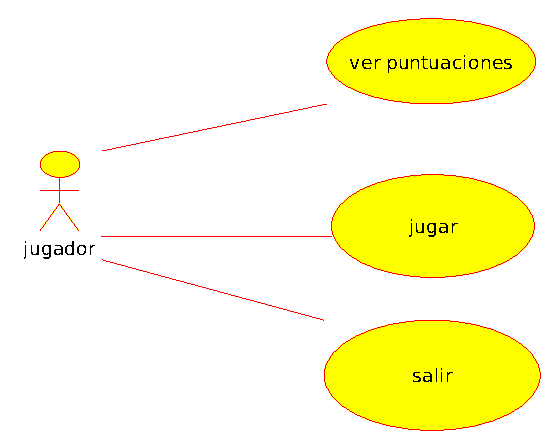
\includegraphics[width = 10 cm]{casos_de_uso_(menu).eps}
\caption{Menú.}
\end{figure}

\begin{figure}[h]
\centering
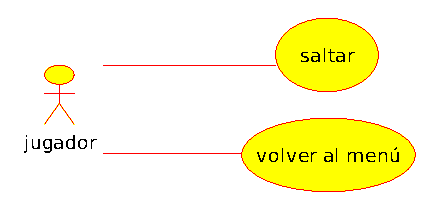
\includegraphics[width = 10 cm]{casos_de_uso_(juego).eps}
\caption{Juego.}
\end{figure}

\clearpage

% -*- coding:utf-8 -*-
\section{Presupuesto}

\begin{itemize}

  \item Costes no recurrentes:

  \begin{itemize}
    \item Registro en Android Market: 18.79 \euro
    \item Equipos portatiles: 4000 \euro (1000 \euro/trabajador, no se incluyen
      para el coste de este proyecto)
    \item Software de desarrollo: 0 \euro (sólo software libre y gratuito)
  \end{itemize}

  \item Costes recurrentes:

  \begin{itemize}

    \item Salario a media jornada: 750 \euro por trabajador/mes

    \begin{itemize}
      \item Sueldo bruto anual: 9000 \euro
      \item Retención IRPF: 0 \euro
      \item Seguridad Social anual: 774.5 \euro
      \item Sueldo Neto anual: 8225.5 \euro
      \item Retención Equivalente: 0 \%
      \item Sueldo neto mensual: 685.46 \euro
      \item Sueldo neto pagas extra: 0 \euro
    \end{itemize}

    \item Proveedor del servicio de internet: 30 \euro por trabajador/mes
    \item Desplazamientos: 40 \euro por trabajador/mes

  \end{itemize}

\end{itemize}

Por tanto, suponiendo un desarrollo a media jornada durante 2 meses, el coste
estimado del proyecto es de {\bf 6578.79 \euro}. Se considera también un fondo
para costes imprevistos de 5000 \euro. Para recuperar la inversión, se
requerirán 7310 descargas a 0.90 \euro.


\section{Trabajo pendiente.}

Finalizar el juego añadiendo los elementos que faltan:

\begin{itemize}
  \item Menú.
  \item Cambio del sprite del jugador.
  \item Si da tiempo, añadir sonido.
\end{itemize}

Añadir a este documento los diagramas que faltan.





\section{fuentes}
http://droideando.blogspot.com.es/2011/03/introduccion-andengine-parte-i.html

\end{document}
